% --- CHUNK_METADATA_START ---
% needs_review: True
% src_checksum: a387e729f92436e818c56320d986498042b8bbec2b20f59a185ece46c35cdd1c
% --- CHUNK_METADATA_END ---
\chapter{Reduction of Endomorphisms}% --- CHUNK_METADATA_START ---
% needs_review: True
% src_checksum: fbc72cfef8a9e5a11acb9fa09f47f0f56fbddd330f7ca5ebbe328e52998a425d
% --- CHUNK_METADATA_END ---
While writing this chapter, I was inspired by the videos of the \textit{3blue1brown} channel which I advise you to watch, at least the playlist concerning linear algebra. The second source of inspiration was Joseph Grifone's book \cite{grifone}.% --- CHUNK_METADATA_START ---
% needs_review: True
% src_checksum: 479ce8267a8dc66449e53b838492edeab11f9f116eed87da087547c1cd388ae6
% --- CHUNK_METADATA_END ---
\section{Introduction}% --- CHUNK_METADATA_START ---
% needs_review: True
% src_checksum: b259dc72d8b683f95181cf362a77427e89eb5f523b8d267844312acf75c8bd32
% --- CHUNK_METADATA_END ---
In the previous chapter, we studied the notion of an orthonormal basis, the utilities of which are: simplification of coordinate calculations in a basis and calculation of a projection. 
This notion is one of the first steps towards the study of SVD\footnote{Singular Value Decomposition} which is applied in several fields, e.g.: the reduction of image sizes.
\par
In this chapter, we continue the study of bases in order to finally understand the SVD. We will study the reduction of endomorphisms, \textit{to be more precise} diagonalization and triangularization. To begin: a small exercise:% --- CHUNK_METADATA_START ---
% needs_review: True
% src_checksum: c724d8f48a016c11bc237e7ac867213a4de62ac70e8e5b7af983c5583736e72b
% --- CHUNK_METADATA_END ---
\begin{ex}
   Calculate
   \[
   \begin{bmatrix} 
       3 & 1\\
       0 & 2
   \end{bmatrix}^{15} = \underbrace{
       \begin{bmatrix} 
       3 & 1\\
       0 & 2
       \end{bmatrix}
       \cdot
       \ldots
       \cdot
       \begin{bmatrix} 
       3 & 1\\
       0 & 2
       \end{bmatrix}
   }_{15 \text{ fois}}
   \] 
\end{ex}% --- CHUNK_METADATA_START ---
% needs_review: True
% src_checksum: db54f58737d8f17d246be0188ca795e38d99b1523ea21594f4d2a50062df2fef
% --- CHUNK_METADATA_END ---
This doesn't seem very easy, does it? At the end of this chapter, we will find a way to simplify the calculation and in the end we will solve this exercise.
\par

We know from linear algebra that we can represent a matrix of a mapping in different bases, i.e. let $\{e_i\}$ be a basis of $E$ and $f$ a mapping. Then this mapping in the basis $\{e_i\}$ is represented:
 \[
A = M(f)_{e_i} = \|f(e_1), \ldots, f(e_n)\|
\]
Let $\{e_i'\}$ be another basis of $E$, then we can represent the mapping $f$ in this basis as well, let's denote: $P = P_{e_i \to e_i'}$ a change-of-basis matrix from the basis% --- CHUNK_METADATA_START ---
% needs_review: True
% src_checksum: a455440085569ccfa50055d0bc7764665730f4c664f1b99eaf1ad4cea3c5ff0c
% --- CHUNK_METADATA_END ---
From $\{e_i\}$ to the base $\{e_i'\}$
 \[
     A' = M(f)_{e_i'} = P^{-1}AP = \|f(e_1'), \ldots, f(e_n')\|_{e_i'}
\]% --- CHUNK_METADATA_START ---
% needs_review: True
% src_checksum: fc62110b6f4665fe0026522308f37adea92af33580b2a7c7add82761c52f764b
% --- CHUNK_METADATA_END ---
\begin{definition}\label{def:matrice-diagonalisable}
    The matrix $A$ is \textbf{diagonalizable} if there exists a similar matrix \footnote{$A$ is similar to $A’$ if there exists a change-of-basis matrix $P$ such that $A’ = P^{-1}AP$}  $A'$ that is diagonal:
     \[
         A' = 
         \begin{bmatrix} 
         a_{1,1} & 0 & \ldots & 0 \\
         0 & a_{2,2} & \ddots & \vdots\\
         \vdots & \ddots & \ddots & 0\\
         0 & \ldots & 0 & a_{n,n}
        \end{bmatrix} 
    \] 
\end{definition}% --- CHUNK_METADATA_START ---
% needs_review: True
% src_checksum: 63bf784efd9f3eb008441c2a262bd3d1b80786b3b1a31a8757b9c25a4783d594
% --- CHUNK_METADATA_END ---
\begin{definition}
    The matrix $A$ is \textbf{triangulable} if there exists a similar triangular (upper/lower) matrix $A'$
     \[
         A' = 
         \begin{bmatrix} 
         a_{1,1} & a_{1,2} & \ldots & a_{1,n} \\
         0 & a_{2,2} & \ddots & \vdots\\
         \vdots & \ddots & \ddots & a_{n-1,n}\\
         0 & \ldots & 0 & a_{n,n}
        \end{bmatrix} \text{ or } 
         A' = 
         \begin{bmatrix} 
         a_{1,1} & 0 & \ldots & 0 \\
         a_{2, 1} & a_{2,2} & \ddots & \vdots\\
         \vdots & \ddots & \ddots & 0\\
         a_{n, 1} & \ldots & a_{n, n-1} & a_{n,n}
        \end{bmatrix} 
    \] 
\end{definition}% --- CHUNK_METADATA_START ---
% needs_review: True
% src_checksum: 5f36cb427b1a26270fb9aa3171f8dc649052df2172578e9eb24535d8e71fd7cf
% --- CHUNK_METADATA_END ---
So the problems in this chapter that we are going to solve are:% --- CHUNK_METADATA_START ---
% needs_review: True
% src_checksum: e36e2423a78b0f5075b2b2706ad1c82fdb9585a3416a6d0dccbc72776563fe3c
% --- CHUNK_METADATA_END ---
\begin{enumerate}
    \item Determine whether an endomorphism $f$ is diagonalizable/triangulable, i.e., if there exists such a matrix $A'$.
    \item Determine the change-of-basis matrix $P$ and the matrix $A'$.
\end{enumerate}% --- CHUNK_METADATA_START ---
% needs_review: True
% src_checksum: 746031095d9367be5953361e604557802b5229ceb1b198f8e1c5eec023f51276
% --- CHUNK_METADATA_END ---
Throughout the chapter, we assume that the vector space $E$ is of finite dimension.% --- CHUNK_METADATA_START ---
% needs_review: True
% src_checksum: f83f4cb55bb9c5b3cbc60c46b58cdb42004864f151f562e6972be1a2ca7cf659
% --- CHUNK_METADATA_END ---
\section{Eigenvectors - Eigenvectors}% --- CHUNK_METADATA_START ---
% needs_review: True
% src_checksum: bfa0ded24a8ac43fd1d9220db52f0511c9dab14b2d78ce78fcafc81151802127
% --- CHUNK_METADATA_END ---
Let's start by clarifying the concept of a linear application and its matrix. Let's take for that the matrix from the exercise at the beginning of the chapter:
\[
A = \begin{bmatrix} 
       3 & 1\\
       0 & 2
   \end{bmatrix}
\] 
This matrix transforms the vector space that we give it, or, to simplify, it transforms each vector of the vector space. Let's take a vector $v_3 = \begin{pmatrix} 1 \\ 1 \end{pmatrix} $, by applying $A$ we obtain:
 \[
Av_3 = \begin{bmatrix} 
       3 & 1\\
       0 & 2
   \end{bmatrix}\begin{bmatrix} 1 \\ 1 \end{bmatrix} = \begin{bmatrix} 3 \\ 0 \end{bmatrix} + \begin{pmatrix} 1 \\ 2 \end{pmatrix} = \begin{bmatrix} 4 \\ 2 \end{bmatrix} 
\]% --- CHUNK_METADATA_START ---
% needs_review: True
% src_checksum: 53748873e68a45b71c636a03328d19fc757a130cd10577ec5dd38db4946a9bc4
% --- CHUNK_METADATA_END ---
\begin{center}
    
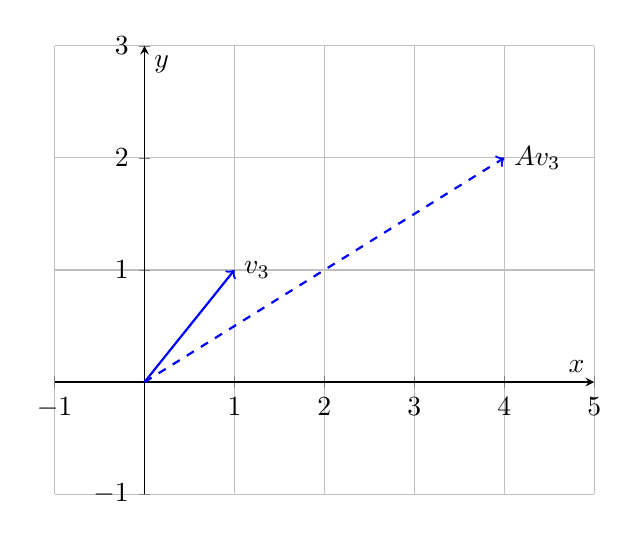
\begin{tikzpicture}
    \begin{axis}[
        axis lines=middle, 
        grid=major, 
        xlabel={$x$}, 
        ylabel={$y$}, 
        ymin=-1, ymax=3,
        xmin=-1, xmax=5
    ]
        % Define original vectors
        \addplot[->, thick, blue] coordinates {(0,0) (1,1)};
        \node[right] at (axis cs:1,1) {$v_3$};

        % Define transformed vectors
        \addplot[->, thick, blue, dashed] coordinates {(0,0) (4,2)};
        \node[right] at (axis cs:4,2) {$A v_3$};
    \end{axis}
\end{tikzpicture}
\end{center}% --- CHUNK_METADATA_START ---
% needs_review: True
% src_checksum: c8eddafdabc468a12a779b174e90bdbbddeb623438e52e27b1a870129d645880
% --- CHUNK_METADATA_END ---
We note that the vector $Av_3$ is no longer located on the same line as the vector $v_3$, which makes sense because if the vectors were on the same lines after a transformation, it would not make sense.
On the other hand, sometimes there are cases when the vector applied to the matrix remains on the same line, for example the vector $v_2 = \begin{pmatrix} -1 \\ 1 \end{pmatrix} $, with $Av_2 = \begin{pmatrix} -2 \\ 2 \end{pmatrix} = 2v_2 $% --- CHUNK_METADATA_START ---
% needs_review: True
% src_checksum: 3f4b5a2eab7d09a193bb48234f784fd0500a5a1563461a78ec7dc45a4abe55d8
% --- CHUNK_METADATA_END ---
\begin{center}
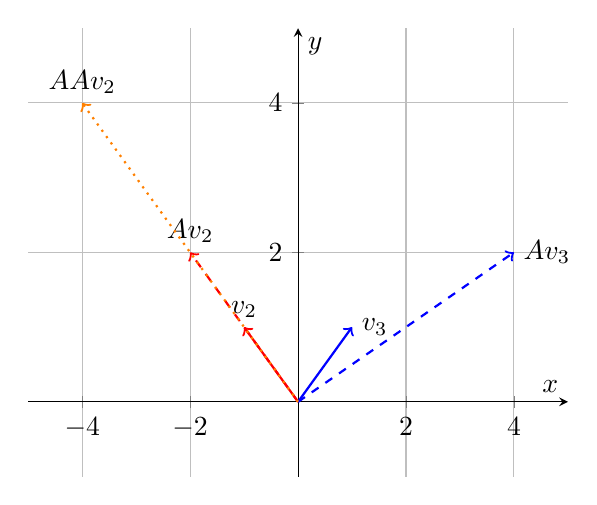
\begin{tikzpicture}
    \begin{axis}[
        axis lines=middle, 
        grid=major, 
        xlabel={$x$}, 
        ylabel={$y$}, 
        ymin=-1, ymax=5,
        xmin=-5, xmax=5
    ]
        % Define original vectors
        \addplot[->, thick, red] coordinates {(0,0) (-1, 1)};
        \node[above] at (axis cs:-1,1) {$v_2$};
        
        \addplot[->, thick, blue] coordinates {(0,0) (1,1)};
        \node[right] at (axis cs:1,1) {$v_3$};

        % Define transformed vectors
        \addplot[->, thick, red, dashed] coordinates {(0,0) (-2,2)};
        \node[above] at (axis cs:-2,2) {$A v_2$};
        
        \addplot[->, thick, blue, dashed] coordinates {(0,0) (4,2)};
        \node[right] at (axis cs:4,2) {$A v_3$};

        % Define transformed vectors
        \addplot[->, thick, orange, dotted] coordinates {(0,0) (-4,4)};
        \node[above] at (axis cs:-4,4) {$A A v_2$};
    \end{axis}
\end{tikzpicture}
\end{center}% --- CHUNK_METADATA_START ---
% needs_review: True
% src_checksum: f0865ddb0d189a62787148c9921474158e89812893ff7f5306eec98881902765
% --- CHUNK_METADATA_END ---
And this is not only the case for the vector $\begin{pmatrix} -1 \\ 1 \end{pmatrix} $, by taking any vector generated by $v = \begin{pmatrix} -1 \\ 1 \end{pmatrix} $, we will obtain $Av = 2v$.
Such vectors $v$ and the scalars (here: 2) are called eigenvectors and eigenvalues respectively. So, we have the formal definition:% --- CHUNK_METADATA_START ---
% needs_review: True
% src_checksum: 6f65d300d8dcb289daa1913b1f3036a9ac4df8dce62a7501a703b883c85b7e50
% --- CHUNK_METADATA_END ---
\begin{definition}
    Let $f$ be an endomorphism in $E$ and a vector $v \in E$ is called an \textbf{eigenvector} of $f$ if:
     \begin{enumerate}
        \item $v \neq 0$
        \item There exists a real number $\lambda$ such that $f(v) = \lambda v$
    \end{enumerate}
    The scalar $\lambda \in \R$ is called the \textbf{eigenvalue} corresponding to $v$.
\end{definition}% --- CHUNK_METADATA_START ---
% needs_review: True
% src_checksum: 8d6f015d17f0abf73d562b2fcade1f9ce8da6e829052fe852d27a804164c13f9
% --- CHUNK_METADATA_END ---
\begin{intuition}
   Eigenvectors are vectors that, under the action of $f$, do not change direction, only length (not even always). This simplifies the calculation of such vectors. Can you calculate $A^3v_3$? Not very easy, then the vector $A^3v_2$? 
   \[
    Av_2 = 2v_2 \implies A^2v_2 = 2\cdot 2v_2 = 4v_2 \implies A^3v_2 = 2 \cdot 4v_2 = 8v_2 = \begin{pmatrix} -8 \\ 8 \end{pmatrix} 
   \] 
   That's cool, isn't it?
\end{intuition}% --- CHUNK_METADATA_START ---
% needs_review: True
% src_checksum: e95160f028b2d95e35269b03fdbba6365717d280a82da361b410a33d65ab24ef
% --- CHUNK_METADATA_END ---
On the other hand, this is not the only use of eigenvectors, and we will come back to discuss it here, but first, how do we find such vectors?% --- CHUNK_METADATA_START ---
% needs_review: True
% src_checksum: 24239d1f10bd0d5f05ad63e362795198d22e9c836bde4895ebccdf0135afeb91
% --- CHUNK_METADATA_END ---
\section{Finding Eigenvalues}% --- CHUNK_METADATA_START ---
% needs_review: True
% src_checksum: 13b0ede61dd64f7dedbca98bbba8400c2c415f0476dbc974f4b86a03654e9e26
% --- CHUNK_METADATA_END ---
We are looking for vectors which, under the action of the endomorphism $f$, are scaled by a factor of $\lambda \in \R$, so we are supposed to solve this equation:% --- CHUNK_METADATA_START ---
% needs_review: True
% src_checksum: 033cd21f2fe1093d7a3b35c11741aa3150ad95a605391060449ea0add1cc2e90
% --- CHUNK_METADATA_END ---
\begin{align*}
    && f(v) &= \lambda v\\
    \iff&& Av &= \lambda v \quad \text{ in matrix notation}\\
    \iff&& Av &= \lambda (Iv) \quad \text{ where } I \text{ is an identity matrix}\\
    \iff&& Av - \lambda Iv &= 0\\
    \iff&& (A - \lambda I)v &= 0
\end{align*}% --- CHUNK_METADATA_START ---
% needs_review: True
% src_checksum: 54fc59c3379c369321a8bd4b11a191dd4e09d3fcc1eeb5bc3ce1eee9d2c9dca2
% --- CHUNK_METADATA_END ---
Therefore, we must study the application $(A - \lambda I)$ and connect it to the notion of determinants. Recall: if the determinant of a matrix is non-zero, then that matrix (i.e., endomorphism) is injective. In our case, if $\det(A - \lambda I)$ were zero, the only vector $v$ that would give $(A - \lambda I)v = 0$ was the zero vector $v = 0$ because $(A - \lambda I)$ is linear and (as we have supposed) injective.
\par
On the other hand, according to the definition, eigenvectors are not zero, so the injective case is not suitable; therefore, to have eigenvectors, the application $(A - \lambda I)$% --- CHUNK_METADATA_START ---
% needs_review: True
% src_checksum: c0eb7dd1aa99ead5c9d932030eaf0651f2dbb1350d1b3b113959c2f476f3c2dd
% --- CHUNK_METADATA_END ---
must not be injective, which is equivalent to saying that $\det(A - \lambda I) = 0$. So, we are supposed to calculate the following determinant:
\[
\det(A - \lambda I) = \det \left(\begin{bmatrix} 
    a_{1,1} & a_{1, 2} & \ldots & a_{1, n}\\
    a_{2,1} & a_{2, 2} & \ldots & a_{2, n}\\
    \ldots & \ldots & \ldots & \ldots\\
    a_{n,1} & a_{n,2} & \ldots & a_{n,n}
    \end{bmatrix}  - 
    \begin{bmatrix} 
        \lambda & 0 & \ldots & 0 \\
        0 & \lambda & \ldots & 0 \\
        \ldots & \ldots & \ldots & \ldots\\
        0 & 0 & \ldots & \lambda
    \end{bmatrix}\right) = 
    \begin{vmatrix} 
    a_{1,1} - \lambda & a_{1, 2} & \ldots & a_{1, n}\\
    a_{2,1} & a_{2, 2} - \lambda & \ldots & a_{2, n}\\
    \ldots & \ldots & \ldots & \ldots\\
    a_{n,1} & a_{n,2} & \ldots & a_{n,n} - \lambda
    \end{vmatrix}
\]% --- CHUNK_METADATA_START ---
% needs_review: True
% src_checksum: 202d0d779c7fd9d48fcaf7cbee2aaf0d018bbf151af905d06eb3a68c0c7a2a52
% --- CHUNK_METADATA_END ---
By expanding this determinant, we obtain an equation of the type:
\[
    (-1)^n\lambda^n + a_{n-1}\lambda^{n-1} + \ldots + a_1\lambda + a_0 = 0
\] 
whose roots are the eigenvalues of $f$ (remember: an eigenvalue is a factor $\lambda$).
Don't focus too much on this equation for now, we'll come back to it.% --- CHUNK_METADATA_START ---
% needs_review: True
% src_checksum: bf5ce8533f46a4f7d3bb2ec19a9531b9c7c84da26177bfd05b62e7f049ee1840
% --- CHUNK_METADATA_END ---
\begin{prop}\label{prop:polynome-caracteristique}
   Let $f$ be an endomorphism in a vector space $E$ of finite dimension $n$ and $A$ the representative matrix of $f$ in a basis of $E$. The eigenvalues of $f$ are the roots of the polynomial:
   \[
   P_f(\lambda) = \det(A - \lambda I)
   \] 
   This polynomial is called the \textbf{characteristic polynomial} of $f$.
\end{prop}% --- CHUNK_METADATA_START ---
% needs_review: True
% src_checksum: 14fc75ccd809e480d739d2a472754a41d41f69e99004bb24fa4505811a704a06
% --- CHUNK_METADATA_END ---
\begin{definition}
    The set of eigenvalues of $f$ is called the \textbf{spectrum} of $f$ and is denoted $\operatorname{Sp}_K(f)$ or $\operatorname{Sp}_K(A)$ if $A$ is a matrix of $f$.
\end{definition}% --- CHUNK_METADATA_START ---
% needs_review: True
% src_checksum: e2c4c99332b07d283c4805a8d6067b3a6eb0885afdafc105915cb259b9b4c138
% --- CHUNK_METADATA_END ---
To clarify:% --- CHUNK_METADATA_START ---
% needs_review: True
% src_checksum: a5e3776b3752e25e079b4a4ff3afc0162901a7b76024cc083b56bfa4e2c66933
% --- CHUNK_METADATA_END ---
\begin{eg}
   Let $f$ be an endomorphism in $\R^2$ whose representative matrix in the canonical basis is:
   \[
       \begin{bmatrix} 3 & 1\\ 0 & 2 \end{bmatrix} 
   \] 
   Let's calculate its eigenvalues:
   \begin{align*}
       && \begin{bmatrix} 3 & 1\\ 0 & 2 \end{bmatrix} v &= \lambda v \\
       \iff && \begin{bmatrix} 3 & 1\\ 0 & 2 \end{bmatrix} v - \lambda I v &= 0\\
       \iff && \left(\begin{bmatrix} 3 & 1\\ 0 & 2 \end{bmatrix}  - \lambda I\right)v  &= 0\\
       \implies && \det \left( \begin{bmatrix} 3 & 1\\ 0 & 2 \end{bmatrix}  - \lambda I \right) &= 0\\
       \implies && \det \left( \begin{bmatrix} 3 & 1\\ 0 & 2 \end{bmatrix}  - \lambda \begin{bmatrix} \lambda & 0\\ 0 & \lambda \end{bmatrix}  \right) &= 0\\
       \implies && \det \left( \begin{bmatrix} 3 - \lambda & 1\\ 0 & 2 - \lambda \end{bmatrix}\right) &= 0\\
                && &= (3-\lambda)(2 - \lambda) = 0
   \end{align*}
   We can clearly see that the solutions are: $\lambda_1 = 3$ and $\lambda_2 = 2$
\end{eg}% --- CHUNK_METADATA_START ---
% needs_review: True
% src_checksum: 745ff8ce1da376f0eac0417d1b613c9bbfdc10a8ac9a92ce5fcf0d22e6c24b88
% --- CHUNK_METADATA_END ---
We can find eigenvalues, nevertheless, we were looking for the \underline{eigenvectors}. And we are there:% --- CHUNK_METADATA_START ---
% needs_review: True
% src_checksum: 76807a4d62a1c1b3f9131c858a7a8e3b4b1c2dd912ab98cfc70831c74c455316
% --- CHUNK_METADATA_END ---
\section{Finding Eigenvectors}% --- CHUNK_METADATA_START ---
% needs_review: True
% src_checksum: b1c16951b8606492536c7b6091686d6ae8882a62f54da1d178856d27e1a5b621
% --- CHUNK_METADATA_END ---
Suppose that for $q \in \N^{*}$ we have already found $q$ eigenvalues of a matrix $\{ \lambda_1, \ldots, \lambda_q \}$, to find the eigenvectors, we still need to find the basis of:
\[
    \ker(A - \lambda_iI) \quad \forall i \in \{1, \ldots, q\}
\] 
which is equivalent to:
\[
\left( A - \lambda_i I \right)v = 0 \quad \forall i \in \{1, \ldots, q\}
\]% --- CHUNK_METADATA_START ---
% needs_review: True
% src_checksum: be6b8287736d668df8afe873cfc7115ccfab543d54d6dba9446182b22675f15e
% --- CHUNK_METADATA_END ---
\begin{eg}
   Again, the matrix  
   \[
       A = \begin{bmatrix} 3 & 1\\ 0 & 2 \end{bmatrix} 
   \] 
   in the canonical basis of $\R^2$. We have already found its eigenvalues: $\lambda_1 = 3$ and $\lambda_2 = 2$. So, let's find the vectors:
   \[
       \begin{bmatrix} 3 - \lambda_1 & 1 \\ 0 & 2 - \lambda_1 \end{bmatrix}\begin{bmatrix} x \\ y \end{bmatrix} = \begin{bmatrix} 3 - 3 & 1 \\ 0 & 2 - 3 \end{bmatrix}\begin{bmatrix} x \\ y \end{bmatrix} = \begin{bmatrix} 0 & 1 \\ 0 & -1 \end{bmatrix}\begin{bmatrix} x \\ y \end{bmatrix} = 0 
       \implies \begin{cases}
           y = 0\\
           -y = 0\\
           x \in \R
       \end{cases}
   \] 
   Therefore, $\ker(A - 3I) = \begin{pmatrix} x \\ 0 \end{pmatrix} =  \operatorname{Vect}(\begin{pmatrix} 1 \\ 0 \end{pmatrix} )$. Here is our first eigenvector: $\begin{pmatrix} 1 \\ 0 \end{pmatrix} $. For the second one:
   \[
       \begin{bmatrix} 3 - \lambda_2 & 1 \\ 0 & 2 - \lambda_2 \end{bmatrix}\begin{bmatrix} x \\ y \end{bmatrix} = \begin{bmatrix} 3 - 2 & 1 \\ 0 & 2 - 2 \end{bmatrix}\begin{bmatrix} x \\ y \end{bmatrix} = \begin{bmatrix} 1 & 1 \\ 0 & 0 \end{bmatrix}\begin{bmatrix} x \\ y \end{bmatrix} = 0 
       \implies \begin{cases}
           x + y = 0
       \end{cases} \implies \begin{cases}
           x = -y
       \end{cases}
   \] 
   Therefore, $\ker(A - 2I) = \begin{pmatrix} -y \\ y \end{pmatrix} = y \begin{pmatrix} -1 \\ 1 \end{pmatrix} = \operatorname{Vect}(\begin{pmatrix} -1 \\ 1 \end{pmatrix} )  $ and here is the second eigenvector: $\begin{pmatrix} -1 \\ 1 \end{pmatrix} $ (it was our vector $v_2$ at the beginning of the chapter).
\end{eg}% --- CHUNK_METADATA_START ---
% needs_review: True
% src_checksum: bfe0ade345d9629ebf9cee9294d50062797294071d549c1785fda381e4a6a15c
% --- CHUNK_METADATA_END ---
Finally, the useful property:% --- CHUNK_METADATA_START ---
% needs_review: True
% src_checksum: b5fe3fa2658dff19e7f53c909d80fba3b08b1479a790a2ef5ddc64002859fde1
% --- CHUNK_METADATA_END ---
\begin{prop}
    Let $A \in \mathcal{M}_n(\R)$ be a matrix with its eigenvectors: $\{\lambda_1, \ldots, \lambda_n\}$, then:
    \begin{align*}
        &\operatorname{Tr}(A) = \lambda_1 + \ldots + \lambda_n\\
        &\operatorname{det}(A) = \lambda_1 \cdot  \ldots \cdot  \lambda_n\\
    \end{align*}
\end{prop}% --- CHUNK_METADATA_START ---
% needs_review: True
% src_checksum: f6522280fbb2a49df36ea182e9cf15e7e5fa21c740e2767f1cb2a283d07f801e
% --- CHUNK_METADATA_END ---
\section{Diagonalizable endomorphisms}% --- CHUNK_METADATA_START ---
% needs_review: True
% src_checksum: 42e680abdbc7cf96f41b775cb88850a76fad72acd49f5231124812d3dff1aa63
% --- CHUNK_METADATA_END ---
Let's revisit the utility of eigenvectors. Let $f$ be an endomorphism of $E$ whose base is $\{e_1, \ldots, e_n\}$ and $\operatorname{Mat}_{e_i}(f) = A$ and the matrix of $f$ in this base. Let's take the following example again:% --- CHUNK_METADATA_START ---
% needs_review: True
% src_checksum: b1bcb0822f0c84465899d760c678f05039f6a3f2d3cddb2242be844e1f59462f
% --- CHUNK_METADATA_END ---
\begin{eg} We have: $A = \begin{bmatrix} 3 & 1\\ 0 & 2 \end{bmatrix} $ in the canonical basis $e_1 = \begin{bmatrix} 1 \\ 0 \end{bmatrix} $ and $e_2 = \begin{bmatrix} 0 \\ 1 \end{bmatrix} $. We recall that we found two eigenvectors:
     \[
     \begin{cases}
         v_1 = \begin{pmatrix} 1 \\ 0 \end{pmatrix} \\
         v_2 = \begin{pmatrix} -1 \\ 1 \end{pmatrix} 
     \end{cases}
     \] 
     We notice that these two vectors are linearly independent and thus form a basis for $\R^2$. Let's try to change the basis of $A$ using two methods:
      \begin{enumerate}
          \item We can calculate the coordinates of $f(v_1)$ and $f(v_2)$ in the basis $\{v_1, v_2\}$, we have:
              \begin{align*}
                  &f(v_1) = 3v_1 = 3 \cdot v_1 + 0 \cdot v_2\\
                  &f(v_2) = 2v_2 = 0 \cdot v_1 + 2 \cdot v_2
              \end{align*}
              And thus $\operatorname{Mat}_{v_i}(f) = \|f(v_1), f(v_2)\|_{v_i} = \begin{bmatrix} 3 & 0 \\ 0 & 2 \end{bmatrix} $ 
          \item We can calculate the change-of-basis matrix $P = P_{e_i \to v_i}$ from the basis $\{e_i\}$ to the basis $\{v_i\}$ and deduce the matrix of $f$ in the new basis. We have:
             \[
            \begin{cases}
                v_1 = \begin{pmatrix} 1 \\ 0 \end{pmatrix} = 1 \cdot e_1 + 0 \cdot e_2 = \begin{pmatrix} 1 \\ 0 \end{pmatrix}_{e_i} \\
                v_2 = \begin{pmatrix} -1 \\ 1 \end{pmatrix} = -1 \cdot e_1 + 1 \cdot e_2 = \begin{pmatrix} -1 \\ 1 \end{pmatrix}_{e_i} \\
            \end{cases}
            \] 
              thus $P = \begin{bmatrix} 1 & -1\\ 0 & 1 \end{bmatrix} $ and $P^{-1} = \begin{bmatrix} 1 & 1 \\ 0 & 1  \end{bmatrix}$ (you can verify the calculation). And so:
              \[
                  A' = P^{-1}AP = \begin{bmatrix} 1 & 1 \\ 0 & 1 \end{bmatrix} \begin{bmatrix} 3 & 1 \\ 0 & 2 \end{bmatrix} \begin{bmatrix} 1 & -1 \\ 0 & 1 \end{bmatrix} = \begin{bmatrix} 1 & 1 \\ 0 & 1 \end{bmatrix} \underbrace{\begin{bmatrix} 3 & -2 \\ 0 & 2 \end{bmatrix}}_{AP} = \begin{bmatrix} 3 & 0 \\ 0 & 2 \end{bmatrix} 
              \] 
     \end{enumerate}
     And there you have it, the magic: we found the diagonal matrix.
\end{eg}% --- CHUNK_METADATA_START ---
% needs_review: True
% src_checksum: 413a1dfd9cd7cd1f178a02fdc7f63469147614941ffcd0311ca8af286d1f8dcf
% --- CHUNK_METADATA_END ---
Next, let's generalize what we have done.% --- CHUNK_METADATA_START ---
% needs_review: True
% src_checksum: 77f963d6a51d6406e8e2c398719648118c2decfe33539ffdaf2d6a2a1de08891
% --- CHUNK_METADATA_END ---
\begin{definition}
    Let $\lambda \in K$, we denote:
    \[
        E_{\lambda} := \{v \in E \mid f(v) = \lambda v \}
    \] 
    $E_{\lambda}$ is a vector space of $E$ called \textbf{eigen-space} corresponding to $\lambda$.
\end{definition}% --- CHUNK_METADATA_START ---
% needs_review: True
% src_checksum: d6263778d0675b5987e98c8bc733dec041940c50bf52f18c63986fecfbfdc82e
% --- CHUNK_METADATA_END ---
\begin{remark}
   \begin{enumerate}
       \item If $\lambda$ is not an eigenvalue of $f$, then $E_\lambda = \{0\}$
       \item If $\lambda$ is an eigenvalue, then:
            \[
                E_\lambda = \{ \text{ eigenvectors associated with } \lambda \} \cup \{0\} \text{ and } \dim E_\lambda \ge 1
           \] 
   \end{enumerate} 
\end{remark}% --- CHUNK_METADATA_START ---
% needs_review: True
% src_checksum: 1267f7e54da5fa5982e2c20354feb1ab54afc84f52353ec7f02a698172136c65
% --- CHUNK_METADATA_END ---
\begin{prop} Let $\lambda_1, \ldots, \lambda_p$ be pairwise distinct scalars. Then the eigenspaces $E_{\lambda_1}, \ldots, E_{\lambda_p}$ form a direct sum. In other words, if $\mathcal{B}_1, \ldots, \mathcal{B}_p$ are bases for $E_{\lambda_1}, \ldots, E_{\lambda_p}$, the family $\{\mathcal{B}_1, \ldots, \mathcal{B}_p\}$ is linearly independent (but not necessarily a spanning set for $E$).
\end{prop}% --- CHUNK_METADATA_START ---
% needs_review: True
% src_checksum: 1379cacc5519b4b0ccc3363240525bcd6703b7b0c2152f3c192d1ac8fdc9fa6f
% --- CHUNK_METADATA_END ---
\begin{preuve}
Let $E_{\lambda_1}, \ldots, E_{\lambda_p}$ be the eigenspaces associated with the eigenvalues $\lambda_1, \ldots, \lambda_p$ of an endomorphism $f$ of a vector space E. We must show that these subspaces are in direct sum, meaning that if a vector belongs to their intersection, then it is zero.

Let's take an element v belonging to their sum, meaning it can be written in the form:
\[
    v = v_1 + v_2 + \cdots + v_p
\]
with $v_i \in E_{\lambda_i}$ for all $i$.

Since each $v_i$ is an eigenvector for $f$ associated with $\lambda_i$, we have:
\[
    f(v_i) = \lambda_i v_i.
\]
Let's apply f to the sum:
\[
    f(v) = f(v_1 + v_2 + \cdots + v_p) = f(v_1) + f(v_2) + \cdots + f(v_p).
\]
Using the linearity of $f$, this gives:
\[
    f(v) = \lambda_1 v_1 + \lambda_2 v_2 + \cdots + \lambda_p v_p.
\]
However, $v$ is also a combination of these same vectors:
\[
    v = v_1 + v_2 + \cdots + v_p.
\]
Therefore, by rearranging:
\[
    (\lambda_1 v_1 + \lambda_2 v_2 + \cdots + \lambda_p v_p) - (v_1 + v_2 + \cdots + v_p) = 0.
\]
Which gives:
\[
    (\lambda_1 - 1) v_1 + (\lambda_2 - 1) v_2 + \cdots + (\lambda_p - 1) v_p = 0.
\]
Let's factor each term:
\[
    (\lambda_1 - \lambda) v_1 + (\lambda_2 - \lambda) v_2 + \cdots + (\lambda_p - \lambda) v_p = 0.
\]
However, the $\lambda_i$ are assumed to be distinct. We deduce that the coefficients are different, and that the sum is zero only if all $v_i$ are zero (since eigenspaces are generally in direct sum).

Thus, $v = 0$, which proves that the eigenspaces are in direct sum.
\end{preuve}% --- CHUNK_METADATA_START ---
% needs_review: True
% src_checksum: 2eaf9f0db0b14b9cd67463a1299269bf5cfef19d7e30ec2ff8476706b6e08893
% --- CHUNK_METADATA_END ---
Thus, the eigenspaces are always in direct sum, but not necessarily equal to $E$:
 \[
     E_{\lambda_1} \oplus \ldots \oplus E_{\lambda_p} \underset{\neq}{\subset} E
\] 
which holds if:
\[
\dim E_{\lambda_1} + \ldots + \dim E_{\lambda_p} < \dim E
\]% --- CHUNK_METADATA_START ---
% needs_review: True
% src_checksum: 8213c21d8868f9e71a42e919a3c73e6db70f4d92487c8f81cd623c0b6a5eff0d
% --- CHUNK_METADATA_END ---
\begin{theorem}
    Let $f$ be an endomorphism in $E$ and $\lambda_1, \ldots, \lambda_p$ its eigenvalues, then the following properties are equivalent:
    \begin{enumerate}
        \item $f$ is diagonalizable
        \item  $E$ is a direct sum of its eigenspaces: $E = E_{\lambda_1} \oplus \ldots \oplus E_{\lambda_p}$
        \item $\dim E_{\lambda_1} + \ldots + \dim E_{\lambda_p} = \dim E$
    \end{enumerate}
\end{theorem}% --- CHUNK_METADATA_START ---
% needs_review: True
% src_checksum: d98bab212106c45f88afcaf4c1d1068a8a038b038282eaa596a01f7a0469250c
% --- CHUNK_METADATA_END ---
\begin{corollary}
   If $f$ is an endomorphism of $E$ with $\dim E = n$ and $f$ admits $n$ pairwise distinct eigenvalues, then $f$ is diagonalizable.
\end{corollary}% --- CHUNK_METADATA_START ---
% needs_review: True
% src_checksum: f46b8c1decbba48b916ea07ecb3f46837dfe2133dcdb857ca960b42272dbc0f2
% --- CHUNK_METADATA_END ---
But since the eigenvalues are the roots of the characteristic polynomial (see prop \ref{prop:polynome-caracteristique}) we have:% --- CHUNK_METADATA_START ---
% needs_review: True
% src_checksum: bc4db3e8c9322d2f54b8b8bd3927f1fecffd46924cbdb8fb78a3872daab6190f
% --- CHUNK_METADATA_END ---
\begin{prop}
    Let $f$ be an endomorphism in $E$ and $\lambda$ an eigenvalue of order $\alpha$ (i.e., $\alpha$ is a root of $P_f(\lambda)$ of order $\alpha$, i.e., $P_f(\lambda) = (X - \lambda)^{\alpha}Q(X)$). Then:
   \[
   \dim E_{\lambda} \le \alpha
   \] 
\end{prop}% --- CHUNK_METADATA_START ---
% needs_review: True
% src_checksum: b41b18de71939fc7ee9fcfc5cfb62fe7bf6f6c45faeef5e2ed2cda68c06cae8e
% --- CHUNK_METADATA_END ---
\begin{theorem}
   Let $f$ be an endomorphism in $E$ with $\dim E = n$. Then $f$ is diagonalizable if and only if:
   \begin{enumerate}
       \item $P_f(X)$ is \underline{split}, i.e:
            \[
                P_f(X) = (-1)^n (X - \lambda_1)^{\alpha_1} \cdot \ldots \cdot (X - \lambda_p)^{\alpha_p}
           \]
           ($\lambda_i$ are the roots, hence the eigenvalues) and $\alpha_1 + \ldots + \alpha_p = n$. Thus, if the sum of the multiplicities of the roots is equal to the dimension of the vector space.
       \item The dimensions of the eigenspaces are \underline{maximal}, i.e $\forall i \in \{1, \ldots, p\}$
           \[
                \dim E_{\lambda_i} = \alpha_i 
           \] 
   \end{enumerate}
\end{theorem}% --- CHUNK_METADATA_START ---
% needs_review: True
% src_checksum: 7bc3254dd77d12e21d0ae0012946c65aae0bce227475ec669ba11498aee3c5b9
% --- CHUNK_METADATA_END ---
\begin{intuition}
   It's not always easy to understand the idea through characteristic polynomials, so another way to look at it is:
   \begin{enumerate}
       \item We find the eigenvalues: $\lambda_1, \ldots, \lambda_p$
       \item Then we find the eigenspaces: $E_{\lambda_i} = \ker(f - \lambda_i I)$
       \item We sum the dimensions: $\dim E_{\lambda_1} + \ldots + \dim E_{\lambda_p} =: d$.  
           \begin{itemize}
               \item 
                   If $d = \dim E$ i.e., if the sum of the dimensions is equal to the dimension of the space  $E$, the eigenspaces span  $E$ and thus  $f$ is diagonalizable (because its matrix can be written in the basis of these eigenvectors).
              \item Otherwise, the number of linearly independent eigenvectors is not sufficient to span  $E$.
           \end{itemize}
   \end{enumerate}
\end{intuition}% --- CHUNK_METADATA_START ---
% needs_review: True
% src_checksum: 1326f78543a8c10e8d45246f66d8ec9489c9aa11bac835c81e13778416517593
% --- CHUNK_METADATA_END ---
\section{Applications}% --- CHUNK_METADATA_START ---
% needs_review: True
% src_checksum: 72ce285d1fc5fa7b57b2a02000cdc6ccee979c0b081f1d7c85b238677961b2ec
% --- CHUNK_METADATA_END ---
\subsection{Calculation of Power}% --- CHUNK_METADATA_START ---
% needs_review: True
% src_checksum: 2c47f2e80bba8d2cda5a17a86a58856e60564538d0253b3fe8dc8251d0fd4b85
% --- CHUNK_METADATA_END ---
\label{subsec:calcule-de-la-puissance-diagonalisation}So, we're back where we started; I remind you of the exercise from the beginning of the chapter:% --- CHUNK_METADATA_START ---
% needs_review: True
% src_checksum: 98d215165627962d168babff6b5f20ceda296a8c477f58a015e756cba56d37a5
% --- CHUNK_METADATA_END ---
\begin{ex} Calculate \[
   \begin{bmatrix} 
       3 & 1\\
       0 & 2
   \end{bmatrix}^{15} = \underbrace{
       \begin{bmatrix} 
       3 & 1\\
       0 & 2
       \end{bmatrix}
       \cdot
       \ldots
       \cdot
       \begin{bmatrix} 
       3 & 1\\
       0 & 2
       \end{bmatrix}
   }_{15 \text{ fois}}
   \] Recall that the eigenvectors of $A$ are: \[
v_1 = \begin{pmatrix} 1 \\ 0 \end{pmatrix} \text{ and } v_2 = \begin{pmatrix} -1 \\ 1 \end{pmatrix} 
\] which are linearly independent and span $\R^2$, thus forming a basis for $\R^2$. Therefore, we can express $A$ in this new basis, and as we have already found:

\[
    A' = P^{-1}AP = \begin{bmatrix} 1 & 1 \\ 0 & 1 \end{bmatrix} \begin{bmatrix} 3 & 1 \\ 0 & 2 \end{bmatrix} \begin{bmatrix} 1 & -1 \\ 0 & 1 \end{bmatrix} = \begin{bmatrix} 3 & 0 \\ 0 & 2 \end{bmatrix} 
\] in the basis $(v_1, v_2)$ with the change-of-basis matrix:
\[
    P = \begin{bmatrix} 1 & -1\\ 0 & 1 \end{bmatrix} \text{ and } P^{-1} = \begin{bmatrix} 1 & 1 \\ 0 & 1  \end{bmatrix}
\] Furthermore, by multiplying $A'$ by $A'$, we get:  
\[
    A' \cdot A' = (P^{-1}AP)(P^{-1}AP) = P^{-1}A^2P = A'^2
\] hence
\[
    A'^n = P^{-1}A^{n}P \implies PA'^nP^{-1} = PP^{-1}A^{n}PP^{-1} = A^{n}
\] This allows us to first calculate the power of $A'$:
 \[
     A'^{15} = \begin{bmatrix} 3 & 0 \\ 0 & 2 \end{bmatrix}^{15} = \begin{bmatrix} 3 & 0 \\ 0 & 2 \end{bmatrix}\begin{bmatrix} 3 & 0 \\ 0 & 2 \end{bmatrix}\begin{bmatrix} 3 & 0 \\ 0 & 2 \end{bmatrix}^{13} = \begin{bmatrix} 3^2 & 0 \\ 0 & 2^2 \end{bmatrix}\begin{bmatrix} 3 & 0 \\ 0 & 2 \end{bmatrix}^{13} = \begin{bmatrix} 3^{15} & 0 \\ 0 & 2^{15} \end{bmatrix}
\] This is much easier than calculating $A^15$ directly, so now we just need to convert back to the canonical basis:
 \[
     P \begin{bmatrix} 3^{15} & 0 \\ 0 & 2^{15} \end{bmatrix} P^{-1} = \begin{bmatrix} 1 & -1 \\ 0 & 1 \end{bmatrix} \begin{bmatrix} 3^{15} & 0 \\ 0 & 2^{15} \end{bmatrix}\begin{bmatrix} 1 & 1 \\ 0 & 1 \end{bmatrix} = \begin{bmatrix} 3^{15} & 3^{15} - 2^{15} \\ 0 & 2^{15}\end{bmatrix} 
\] 
\end{ex}% --- CHUNK_METADATA_START ---
% needs_review: True
% src_checksum: fe7f464ebe9b9b8d70da5869d4f76579874d5b94c94de63f119293e5da5d8801
% --- CHUNK_METADATA_END ---
What is very useful about diagonal matrices is that the power of such a matrix is equal to the same matrix with its diagonal elements raised to the power, i.e:
\[
    A' = \begin{bmatrix} 
        \lambda_1 & 0 & \ldots & 0\\ 
        0 & \lambda_2 & \ldots & 0\\
        \vdots & \ddots & \ddots & \vdots\\
        0 & 0 & \ldots & \lambda_n
    \end{bmatrix} \implies A'^{n} = \begin{bmatrix} 
        \lambda_1 & 0 & \ldots & 0\\ 
        0 & \lambda_2 & \ldots & 0\\
        \vdots & \ddots & \ddots & \vdots\\
        0 & 0 & \ldots & \lambda_n
    \end{bmatrix}^{n} = \begin{bmatrix} 
        \lambda_1^n & 0 & \ldots & 0\\ 
        0 & \lambda_2^n & \ldots & 0\\
        \vdots & \ddots & \ddots & \vdots\\
        0 & 0 & \ldots & \lambda_n^n
    \end{bmatrix}
\]
% --- CHUNK_METADATA_START ---
% needs_review: True
% src_checksum: 8a1a211ead2bc7122b6dabe42a2f9a4a77824ff8ff678c01c28a0219c7f3bf24
% --- CHUNK_METADATA_END ---
Let's generalize: If $A \in \mathcal{M}_n(K)$ is diagonalizable (i.e., there exists $P$ and $A'$ such that $A' = P^{-1}AP$), then:
\[
    A^{n} = P(A'^{n})P^{-1} = P\begin{bmatrix} 
        \lambda_1^n & 0 & \ldots & 0\\ 
        0 & \lambda_2^n & \ldots & 0\\
        \vdots & \ddots & \ddots & \vdots\\
        0 & 0 & \ldots & \lambda_n^n
    \end{bmatrix}P^{-1}
\]% --- CHUNK_METADATA_START ---
% needs_review: True
% src_checksum: 0e437a1301fed7ad8c86c2050cb39354834ce1067ee3e550b442feeadd27f605
% --- CHUNK_METADATA_END ---
\subsection{Resolution of a System of Recurrent Sequences}% --- CHUNK_METADATA_START ---
% needs_review: True
% src_checksum: 61179ab696df148ddf63af38db970e87fbd159d69d175581f925dd5acc35398f
% --- CHUNK_METADATA_END ---
Let $(u_n)_{n \in \N}$ and $(v_n)_{n \in \N}$ be two sequences such that:% --- CHUNK_METADATA_START ---
% needs_review: True
% src_checksum: de0dceb52bfd9f918bccc3dd4b682cbba493b8cd50ec24359e279937e5d57606
% --- CHUNK_METADATA_END ---
\begin{equation}\label{eq:systeme-appli-diagonalisation}
    \begin{cases}
        u_{n+1} = u_n - v_n\\
        v_{n+1} = 2u_n + 4v_n
    \end{cases}
\end{equation}% --- CHUNK_METADATA_START ---
% needs_review: True
% src_checksum: 7fec7b322265c7dbde89c8e55f970aa29a332bc2f44a1e10beeebc20b7e4b2ec
% --- CHUNK_METADATA_END ---
with $u_0 = 2$ and $v_n = 1$. Let $X_n = \begin{pmatrix} u_n \\ v_n \end{pmatrix} $, then the system \ref{eq:systeme-appli-diagonalisation} is written:
\[
    X_{n+1} = AX_n \quad \text{ with } \quad A = \begin{pmatrix} 1 & -1\\ 2 & 4 \end{pmatrix} 
\] 
by recurrence we obtain:
\[
X_n = A^nX_0 \quad \text{ with } X_0 = \begin{pmatrix} 2 \\ 1 \end{pmatrix} 
\] 

So, we are reduced to calculating the power of a matrix: $A^n$ which we saw in section ~\ref{subsec:calcule-de-la-puissance-diagonalisation}. You can check that there exists $P \in GL_2(\R)$ s.t.
\[
    P = \begin{pmatrix} -1 & 1 \\ 1 & -2 \end{pmatrix} \quad \text{ with } \quad A = P\begin{pmatrix} 2 & 0 \\ 0 & 3 \end{pmatrix}P^{-1}
\]% --- CHUNK_METADATA_START ---
% needs_review: True
% src_checksum: 399bd40803e1ba4f375e06ea5e849952aa0e88c744243cac3af98ee3d38235ea
% --- CHUNK_METADATA_END ---
and then
\[
    A^n = P\begin{pmatrix} 2^n & 0 \\ 0 & 3^n \end{pmatrix}P^{-1} = \begin{pmatrix} -1 & 1 \\ 1 & -2 \end{pmatrix}  \begin{pmatrix} 2^n & 0 \\ 0 & 3^n \end{pmatrix}  \begin{pmatrix} -2 & -1 \\ -1 & -1 \end{pmatrix}  =  
    \begin{pmatrix}
        2 \cdot 2^n - 3^n & 2^n - 3^n \\
        -2 \cdot 2^n + 2 \cdot 3^n & -2^n + 2 \cdot 3^n
    \end{pmatrix}
\]
Whence
\[
\begin{pmatrix} u_n \\ v_n \end{pmatrix} = 
    \begin{pmatrix}
        2 \cdot 2^n - 3^n & 2^n - 3^n \\
        -2 \cdot 2^n + 2 \cdot 3^n & -2^n + 2 \cdot 3^n
    \end{pmatrix}
    \begin{pmatrix} 2 \\ 1 \end{pmatrix} 
    =
    \begin{pmatrix}
        4 \cdot 2^n - 2 \cdot 3^n + 2^n - 3^n \\
        -4 \cdot 2^n + 4 \cdot 3^n -2^n + 2 \cdot 3^n
    \end{pmatrix}
\]% --- CHUNK_METADATA_START ---
% needs_review: True
% src_checksum: a751678f651c005345b96ade9b58368b8905ec6236a1edddaa56e81128fe35b1
% --- CHUNK_METADATA_END ---
that is to say:
\[
\begin{cases}
   u_n = 5 \cdot 2^n - 3\cdot 3^n \\
   v_n = -5 \cdot 2^n + 6\cdot 3^n
\end{cases}
\]% --- CHUNK_METADATA_START ---
% needs_review: True
% src_checksum: 51a5b9793de6a99fd33ee7c81e1491ae1e9ccbf2004615c9f851b9ba72e5294a
% --- CHUNK_METADATA_END ---
\subsection{Solving Differential Equations}% --- CHUNK_METADATA_START ---
% needs_review: True
% src_checksum: 5cfb44f1b46d0da82fbb09a6e3232ed56144a2d940ad6004c1c99f8c85a6677c
% --- CHUNK_METADATA_END ---
Consider solving the differential system
\[
\left\{
\begin{aligned}
\frac{dx_1}{dt} &= a_{11}x_1 + \cdots + a_{1n}x_n \\
&\vdots \\
\frac{dx_n}{dt} &= a_{n1}x_1 + \cdots + a_{nn}x_n
\end{aligned}
\right.
\]
with \( a_{ij} \in \mathbb{R} \) and \( x_i : \mathbb{R} \rightarrow \mathbb{R} \) differentiable.\\

In matrix form, the system is written as:% --- CHUNK_METADATA_START ---
% needs_review: True
% src_checksum: 144da0e3d872899bbd35be5d0ee7d39080596dbed466a89e9ebf93a920545227
% --- CHUNK_METADATA_END ---
\begin{equation}\label{eq:equation-differentielle-diagonalisation}
\frac{dX}{dt} = AX, \quad \text{where} \quad A = (a_{ij}), \quad X = 
\begin{pmatrix}
x_1 \\
\vdots \\
x_n
\end{pmatrix}
\end{equation}% --- CHUNK_METADATA_START ---
% needs_review: True
% src_checksum: e601365c81ae29ac547a15dbc56823b5925b90526752ac2c10d6a807daa5f09d
% --- CHUNK_METADATA_END ---
Suppose \( A \) is diagonalizable. Then there exist \( A' \) a diagonal matrix and \( P \) an invertible matrix such that: 
\[
A' = P^{-1}AP.
\]
If \( A \) is considered as the matrix of an endomorphism in the canonical basis, then \( A' \) is the matrix of \( f \) in the basis of eigenvectors \( \{v_i\} \).\\
Likewise, \( X \) is the matrix of a vector \( \vec{x} \) in the canonical basis and \( X' = M(\vec{x})_{v_i} \) is related to \( X \) by
\[
X' = P^{-1}X
\]% --- CHUNK_METADATA_START ---
% needs_review: True
% src_checksum: 3b0f6fa98bbaeac09505e81d4fd1bf0756f609c5a667d816bbd1b588d70d4f8b
% --- CHUNK_METADATA_END ---
\begin{note} Note! In this section $X'$ does not describe the derivative, but a vector denoted $X'$! \end{note}% --- CHUNK_METADATA_START ---
% needs_review: True
% src_checksum: 5989d5a119a0c6c75a347c9d875129aacb6398c3b7a5c5abc15d16de482e34bb
% --- CHUNK_METADATA_END ---
By deriving this relation:
\[
\frac{dX'}{dt} = P^{-1} \frac{dX}{dt}
\]
(because \( A \) having constant coefficients, \( P \) will also have constant coefficients). Therefore:
\[
\frac{dX'}{dt} = P^{-1}AX = \left( P^{-1}AP \right) X' = A'X'
\]
The system \ref{eq:equation-differentielle-diagonalisation} is therefore equivalent to the system
\[
\frac{dX'}{dt} = A'X'
\]

This system is easily integrated, because \( A' \) is diagonal.\\
Thus, we can solve the system \( \frac{dX}{dt} = AX \) in the following way:% --- CHUNK_METADATA_START ---
% needs_review: True
% src_checksum: 82c573543a39f219c01ad57688e75f0bb2d5232a34af85c358773c9165fabfc8
% --- CHUNK_METADATA_END ---
\begin{enumerate}
    \item We diagonalize \( A \). Let \( A' = P^{-1}AP \) be a diagonal matrix similar to \( A \);
    \item we integrate the system \( \frac{dX'}{dt} = A'X' \);
    \item we return to \( X \) using \( X = PX' \).
\end{enumerate}% --- CHUNK_METADATA_START ---
% needs_review: True
% src_checksum: 559d05d3e2e4f1bc31900766c7553059133f5f084e7bfcf1189b2c9c351e9b04
% --- CHUNK_METADATA_END ---
\subsection{Example}% --- CHUNK_METADATA_START ---
% needs_review: True
% src_checksum: f99078a05ae06ddd39a61aa5a948847bed9724a2ac3862a6a0fec135a4a1e884
% --- CHUNK_METADATA_END ---
Consider the system
\[
\left\{
\begin{aligned}
\frac{dx}{dt} &= x - y \\
\frac{dy}{dt} &= 2x + 4y
\end{aligned}
\right.
\]

We have \( A' = \begin{pmatrix} 2 & 0 \\ 0 & 3 \end{pmatrix} \) and 
\( P = \begin{pmatrix} 1 & 1 \\ -1 & -2 \end{pmatrix} \)

The system \( \frac{dX'}{dt} = A'X' \) is written as:
\[
\left\{
\begin{aligned}
\frac{dx'}{dt} &= 2x' \\
\frac{dy'}{dt} &= 3y'
\end{aligned}
\right.
\]
which immediately gives 
\[
\left\{
\begin{aligned}
x' &= C_1 e^{2t} \\
y' &= C_2 e^{3t}
\end{aligned}
\right.
\]
and thus, by reverting to \( X \) using \( X = PX' \) :
\[
\begin{pmatrix}
x \\
y
\end{pmatrix}
=
\begin{pmatrix}
1 & 1 \\
-1 & -2
\end{pmatrix}
\begin{pmatrix}
C_1 e^{2t} \\
C_2 e^{3t}
\end{pmatrix}
=
\begin{pmatrix}
C_1 e^{2t} + C_2 e^{3t} \\
- C_1 e^{2t} - 2C_2 e^{3t}
\end{pmatrix}
\]% --- CHUNK_METADATA_START ---
% needs_review: True
% src_checksum: 5b4cd1ca5148b5fd96a202c46a2ad95c69ac874f8a1550c14f52cc84385c4932
% --- CHUNK_METADATA_END ---
that is to say:
\[
\left\{
\begin{aligned}
x &= C_1 e^{2t} + C_2 e^{3t} \\
y &= -C_1 e^{2t} - 2C_2 e^{3t}
\end{aligned}
\right.
\]% --- CHUNK_METADATA_START ---
% needs_review: True
% src_checksum: c65a4568a9bcb1844020af7eaf577b7f39ff96aea420cb009b9514cef08d44e3
% --- CHUNK_METADATA_END ---
\section{Trigonalization}% --- CHUNK_METADATA_START ---
% needs_review: True
% src_checksum: 4ab1418d7b12b3f4e6303df3c355fd14fc58d0b443d59d177eb4683d084ab4da
% --- CHUNK_METADATA_END ---
A matrix $A \in \mathcal{M}_n(K)$ is called upper triangular if it is of the form:
\[
         A = 
         \begin{bmatrix} 
         a_{1,1} & a_{1,2} & \ldots & a_{1,n} \\
         0 & a_{2,2} & \ddots & \vdots\\
         \vdots & \ddots & \ddots & a_{n-1,n}\\
         0 & \ldots & 0 & a_{n,n}
        \end{bmatrix}
\] 
respectively lower triangular:
\[
         A = 
         \begin{bmatrix} 
         a_{1,1} & 0 & \ldots & 0 \\
         a_{2, 1} & a_{2,2} & \ddots & \vdots\\
         \vdots & \ddots & \ddots & 0\\
         a_{n, 1} & \ldots & a_{n, n-1} & a_{n,n}
        \end{bmatrix} 
\]% --- CHUNK_METADATA_START ---
% needs_review: True
% src_checksum: 1a9f8e217fd2ce5fe57e80db261a3ee285f582c5e903296a18aefb70dab8805c
% --- CHUNK_METADATA_END ---
\begin{remark}
   Any upper triangular matrix $A$ is similar to a lower triangular matrix. 
\end{remark}% --- CHUNK_METADATA_START ---
% needs_review: True
% src_checksum: b5b5d8a6405c91bd12df0edf3a4eb709e0114413918e50c6fbe34c96170f4d63
% --- CHUNK_METADATA_END ---
\begin{proof} Let $A$ be an upper triangular matrix and $f$ be the endomorphism of $K^n$ which, in the basis $\{e_1, \ldots, e_n\}$, is represented by the matrix $A$, then: \[
    \begin{cases}
        f(e_1) = a_{1, 1} e_1\\
        f(e_2) = a_{1, 2} e_1 + a_{2, 2}e_2\\
        \vdots \\
        f(e_n) = a_{1, n} e_1 + a_{2, n}e_2 + \ldots + a_{n, n}e_n
    \end{cases} 
    \iff
         A = 
         \begin{bmatrix} 
         a_{1,1} & a_{1,2} & \ldots & a_{1,n} \\
         0 & a_{2,2} & \ddots & \vdots\\
         \vdots & \ddots & \ddots & a_{n-1,n}\\
         0 & \ldots & 0 & a_{n,n}
        \end{bmatrix}
    \] Let's consider the basis \[
    \varepsilon_1 = e_n, \quad \varepsilon_2 = e_{n-1}, \quad \ldots, \quad \varepsilon_n = e_1
    \] then we have: \[
    \begin{cases}
        f(\underbrace{\varepsilon_1}_{e_n}) = = a_{1, n}\underbrace{\varepsilon_n}_{e_1} + a_{2, n}\underbrace{\varepsilon_{n-1}}_{e_2} + \ldots + a_{n, n}\underbrace{\varepsilon_1}_{e_n} \\
        f(\underbrace{\varepsilon_2}_{e_{n-1}}) = = a_{1, n-1}\underbrace{\varepsilon_n}_{e_1} + \ldots + a_{n-1, n-1}\underbrace{\varepsilon_2}_{e_{n-1}} \\
        \vdots \\
        f(\underbrace{\varepsilon_n}_{e_1}) = a_{1,1}\underbrace{\varepsilon_n}_{e_1}
    \end{cases}
    \] thus \[
    A' = M(f)_{\varepsilon_{i}} = 
    \begin{bmatrix} 
        a_{n, n}   &              & \ldots & 0\\
        a_{n-1, n} & a_{n-1, n-1} & \ldots & 0\\
        \vdots     &              & \ddots & \\
        a_{1, n}   & \ldots       &        & a_{1,1}
    \end{bmatrix} 
    \] 
\end{proof}% --- CHUNK_METADATA_START ---
% needs_review: True
% src_checksum: 37460fab9573e33d85fa8ae192ffa26232cc8f6a421f019fea62542b11d8f8af
% --- CHUNK_METADATA_END ---
\subsection{The geometric intuition of diagonalization}% --- CHUNK_METADATA_START ---
% needs_review: True
% src_checksum: a1b0b06975fef25c28bcda6c003784c7d1dec60e9bb3e3db4ab3d8120c200e6f
% --- CHUNK_METADATA_END ---
Let's recall diagonalization. The matrix $A$ representing the endomorphism $f$ in $K^n = \operatorname{Vect}(e_1, \ldots, e_n)$ is diagonalizable if there exist enough vector subspaces $\{F_1, \ldots, F_n\}$, each of dimension $1$, such that $K^n = F_1 \oplus \ldots \oplus F_n$ and $\forall i \in \{1, \ldots, n\}, f(F_i) \subset F_i$ (a vector remains in the space after applying $f$). What can be seen geometrically:% --- CHUNK_METADATA_START ---
% needs_review: True
% src_checksum: e978070e1f65118ae3801786948dd78b3784251b18bd77ac83163f0112ff7343
% --- CHUNK_METADATA_END ---
\begin{center}
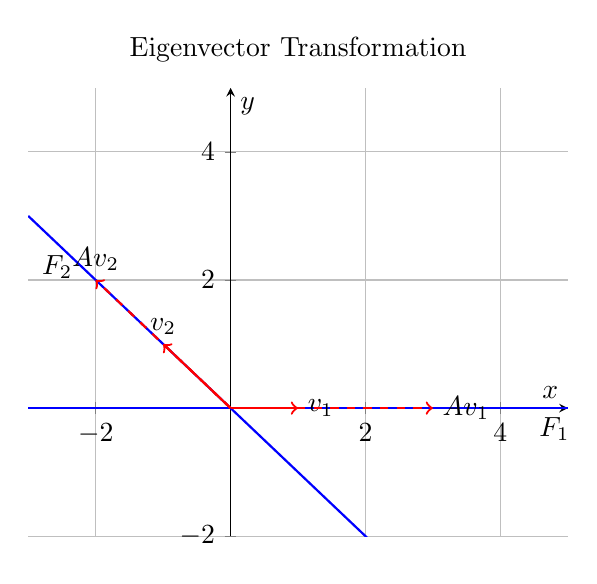
\begin{tikzpicture}
    \begin{axis}[
        axis lines=middle, 
        grid=major, 
        xlabel={$x$}, 
        ylabel={$y$}, 
        title={Eigenvector Transformation},
        ymin=-2, ymax=5,
        xmin=-3, xmax=5
    ]
        \addplot[thick, blue] coordinates {(-3, 0) (5, 0)};
        \node[below] at (axis cs:4.8,0) {$F_1$};

        \addplot[thick, blue] coordinates {(-3,3) (5, -5)};
        \node[below, left] at (axis cs:-2.2,2.2) {$F_2$};

        % Define original vectors
        \addplot[->, thick, red] coordinates {(0,0) (1,0)};
        \node[right] at (axis cs:1,0) {$v_1$};

        \addplot[->, thick, red] coordinates {(0,0) (-1, 1)};
        \node[above] at (axis cs:-1,1) {$v_2$};

        % \addplot[->, thick, blue] coordinates {(0,0) (1,1)};
        % \node[right] at (axis cs:1,1) {$v_3$};
        %
        % \addplot[->, thick, blue] coordinates {(0,0) (-1,2)};
        % \node[left] at (axis cs:-1,2) {$v_4$};

        % Define transformed vectors
        \addplot[->, thick, red, dashed] coordinates {(0,0) (3,0)};
        \node[right] at (axis cs:3,0) {$A v_1$};

        \addplot[->, thick, red, dashed] coordinates {(0,0) (-2,2)};
        \node[above] at (axis cs:-2,2) {$A v_2$};

        %
    \end{axis}
\end{tikzpicture}
\end{center}% --- CHUNK_METADATA_START ---
% needs_review: True
% src_checksum: 61ca3dd1f0de049e0bbd719bb21cc250f384d66f43f47527866160c43e5cc06a
% --- CHUNK_METADATA_END ---
We already know that such an endomorphism is very useful, but it is not often that it can be diagonalized. Therefore, it would be useful to have something more general but still similar to diagonalization.% --- CHUNK_METADATA_START ---
% needs_review: True
% src_checksum: 2968fdfbc22e60619ee8acc09847a6bd93bf80034936aeb0bd1ddf1f3082f359
% --- CHUNK_METADATA_END ---
\subsection{The Geometric Intuition of Trigonalization}% --- CHUNK_METADATA_START ---
% needs_review: True
% src_checksum: 1e27ecfce9650c6586e60226e1a0ca8081f1bd73027a688859e08f85162a7f99
% --- CHUNK_METADATA_END ---
The geometry of the trigonalizable endomorphism is similar yet still different. Let $A$ be a representative matrix of the endomorphism $f$ in $K^n$. It is trigonalizable if there exists a basis $\{v_1, \ldots, v_n\}$ of $K^n$, let's denote $F_1 = \operatorname{Vect}(v_1), F_2 = \operatorname{Vect}(v_1, v_2), \ldots, F_n = \operatorname{Vect}(v_1, v_2, \ldots, v_n)$ such that
\[
F_1 \subset F_2 \subset \ldots \subset F_n
\] 
and 
\[
    \forall i \in \{1, \ldots, n\}, f(F_i) \subset F_i
\] 
Do you see the similarity? The endomorphism is stable by the subspace! The vector applied to $f$ never leaves its subspace. Let's take the following matrix as an example:% --- CHUNK_METADATA_START ---
% needs_review: True
% src_checksum: e0a14bb8ca3479d48070ca15931d4b49951ff405eefc98516a49a7b727dc488d
% --- CHUNK_METADATA_END ---
\[
    A = \begin{bmatrix} 
        1 & 1 & 0\\
        0 & 2 & 1\\
        0 & 0 & 3
    \end{bmatrix} = \operatorname{Mat}(f)_{e_i}
\] 
%  \[
%  \begin{cases}
%      v_1 := \begin{pmatrix} 2 \\ 0 \\ 0 \end{pmatrix} \in F_1, f(\begin{pmatrix} 2 \\ 0 \\ 0 \end{pmatrix}) = \begin{pmatrix} 2 \\ 0 \\ 0 \end{pmatrix} \in F_1\\
%      v_2 = 
%  \end{cases}
%  \]
% --- CHUNK_METADATA_START ---
% needs_review: True
% src_checksum: 4ac6b4fd334aea8ad055545fd6361209311d5ec57c8f10f47b1a293847f5ebe4
% --- CHUNK_METADATA_END ---
\begin{center}
    
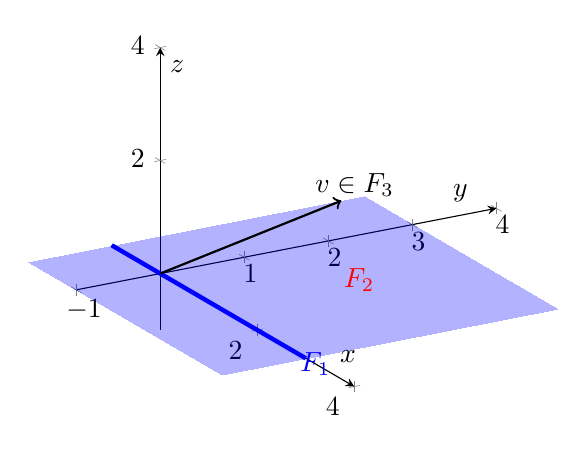
\begin{tikzpicture}
  \begin{axis}[
      view={60}{30},
      axis lines=center,
      xlabel={$x$},
      ylabel={$y$},
      zlabel={$z$},
      xmin=-1, xmax=4,
      ymin=-1, ymax=4,
      zmin=-1, zmax=4,
      samples=10,
      domain=-1:4,
      y domain=-1:4,
      z buffer=sort,
      width=10cm, height=8cm,
  ]
    % F1: Invariant line (x-axis)
    \addplot3[blue, ultra thick, domain=-1:3]({x},{0},{0});
    \node[blue] at (axis cs:3.2,0,0) {$F_1$};

    % \addplot3[->, black, thick] coordinates {(0, 0, 0) (2, 0, 0)};
    % \node[black, above] at (axis cs:2,0,0) {$v_1 = f(v_1)$};

    % F2: Invariant plane (xy-plane)
    \addplot3[
      surf,
      fill=red,
      opacity=0.3,
      shader=interp,
      samples=2,
      domain=-1:3,
      y domain=-1:3,
    ]
    ({x},{y},{0});
    \node[red] at (axis cs:1.5,1.5,0.2) {$F_2$};

    % Optionally: Draw a vector in F3 (illustrating the full space)
    \addplot3[black,->,thick] coordinates {(0,0,0) (2,1,2)};
    \node at (axis cs:2.1,1.1,2.3) {$v\in F_3$};

  \end{axis}
\end{tikzpicture}
\end{center}% --- CHUNK_METADATA_START ---
% needs_review: True
% src_checksum: 8cca275d57768137e37d787409628be302ecf03d302e568627928744fb85d595
% --- CHUNK_METADATA_END ---
As we have an intuition for trigonalizable endomorphisms, let's return to pure mathematics.% --- CHUNK_METADATA_START ---
% needs_review: True
% src_checksum: a5db95e707fd8e6c77bc25fe420465e168c8220a57713ec7934ac000630976f2
% --- CHUNK_METADATA_END ---
\subsection{Theory}% --- CHUNK_METADATA_START ---
% needs_review: True
% src_checksum: 36d1aae4a5b73157818018621c793b8b2714c671bc34e81fa36b07a1c002e80a
% --- CHUNK_METADATA_END ---
\begin{theorem}\label{thm:trigonalisable-si-scinde}
    An endomorphism is trigonalizable in $K$ if and only if its characteristic polynomial splits in $K$. 
    \par 
    This means that the characteristic polynomial has exactly $n$ roots, where $n = \dim(E)$, and can be written as:
     \[
         P_f(X) = (-1)^n(X - \lambda_1)^{\alpha_1}\cdots(X - \lambda_p)^{\alpha_p}
    \] 
    with $\alpha_1 + \ldots + \alpha_p = n$
\end{theorem}% --- CHUNK_METADATA_START ---
% needs_review: True
% src_checksum: f27effc0e9df354b6ed9cf4b3da8028d3743bdcc47f10cfccbc3f5af24a25ec6
% --- CHUNK_METADATA_END ---
\begin{preuve} -
   \begin{itemize}
       \item Suppose the endomorphism $f$ is trigonalizable and let $\{e_1, \ldots, e_n\}$ be a basis such that
           \[
               M(f)_{e_i} = \begin{pmatrix} 
                   a_{1,1} &            & & *\\
                   0       & a_{2, 2}   & & \\
                   \vdots  &      & \ddots & \\
                   0        & \ldots    & 0 & a_{n, n}
               \end{pmatrix} 
           \]
           We have:
           \[
            P_f(X) = \det \begin{pmatrix} 
                   a_{1,1} - X &            & & *\\
                   0       & a_{2, 2} - X   & & \\
                   \vdots  &      & \ddots & \\
                   0        & \ldots    & 0 & a_{n, n} - X
               \end{pmatrix} = (a_{1,1} - X) \cdots (a_{n,n} - X)
           \]
           Thus, $P_f(X)$ is split (we can note that its roots are the eigenvalues of $f$).
       \item Suppose $P_f(X)$ is split and let us show by induction that $f$ is trigonalizable.
            \par
            For $n=1$, it is trivial.
            \par
            Suppose that the result holds for order $n-1$. Since $P_f(X)$ is split, it admits at least one root $\lambda_1 \in K$ and thus an eigenvector $\varepsilon_1 \in E_{\lambda_1}$. Let's complete $\{\varepsilon_1\}$ to a basis $\{\varepsilon_1, \ldots, \varepsilon_n\}$, so we have:
            \[
            A = M(f)_{\varepsilon_i} = \begin{pmatrix} 
                \lambda_1 & b_2 & \ldots & b_n\\
                0         &     &        &    \\
                \vdots    &     & B      &    \\
                0         &     &        &
            \end{pmatrix}, \quad \text{where: } B \in \mathcal{M}_{n-1}(K)
            \]
            Let $F = \operatorname{Vect}(\varepsilon_2, \ldots, \varepsilon_n)$ and $g: F \to F$ be the unique endomorphism of $F$ such that $M(g)_{\varepsilon_2, \ldots, \varepsilon_n} = B$, we have:
            \[
            P_f(X) = \det(A - XI_n) = (\lambda_1 - X)\det(B - XI_{n-1}) = (\lambda_1 - X)P_g(X)
            \]
            Since $P_f(X)$ is split, $P_g(X)$ is also split, and by the induction hypothesis, $B$ is trigonalizable, so there exists a basis $\{v_2, \ldots, v_n\}$ in which $M(g)_{v_2, \ldots, v_n}$ is triangular, and thus the matrix of $f$ in the basis $\{\varepsilon_1, v_2, \ldots, v_n\}$ is triangular, so $f$ is trigonalizable.
   \end{itemize} 
\end{preuve}% --- CHUNK_METADATA_START ---
% needs_review: True
% src_checksum: 9bb744e88dd97bc7d0ae2ea03d3215bcd3fccc78c15bc8f09bcfacaf14071d84
% --- CHUNK_METADATA_END ---
\begin{corollary}
    Any matrix $A \in \mathcal{M}_n(\mathbb{C})$ is similar to a triangular matrix in $\mathcal{M}_n(\mathbb{C})$.
\end{corollary}% --- CHUNK_METADATA_START ---
% needs_review: True
% src_checksum: a3b598c9377193bbd0acace6e3dff04e1b8fd3d50b29e18abeea54d26e5ab17c
% --- CHUNK_METADATA_END ---
\begin{intuition}
    According to the abstract algebra course, every polynomial in $\mathbb{C}$ is split. 
\end{intuition}% --- CHUNK_METADATA_START ---
% needs_review: True
% src_checksum: 23b673348e1d58c00e761620ff4fbfd71672707c2d007e5abd7f154f1199b206
% --- CHUNK_METADATA_END ---
\begin{remark}-
   \begin{enumerate}
       \item If $A$ is trigonalizable and $A'$ is triangularly similar to $A$, then $A'$ has its eigenvalues on the diagonals.
       \item Any matrix $A \in \mathcal{M}_n(K)$ is trigonalizable over the closure $K'$ of $K$. (e.g.: $A \in \mathcal{M}_n(\R)$ is trigonalizable over $\mathbb{C}$).
   \end{enumerate} 
\end{remark}% --- CHUNK_METADATA_START ---
% needs_review: True
% src_checksum: e9bf0c73c0a303936ab15442415a5c043bc85a10dfc78a9f1f25a77c3a1ef9ea
% --- CHUNK_METADATA_END ---
\begin{corollary}
    Let $A \in \mathcal{M}_n(K)$ have $\{\lambda_1, \ldots, \lambda_n\}$ as its eigenvalues, then
    \begin{align*}
        \operatorname{Tr}(A) = \lambda_1 + \ldots + \lambda_n\\
        \det(A) = \lambda_1 \cdot \ldots \cdot  \lambda_n
    \end{align*}
\end{corollary}% --- CHUNK_METADATA_START ---
% needs_review: True
% src_checksum: 6a64df61bb2708a9fd24ca53aed335fb8a45d67e1e7546c637a7189e188878fe
% --- CHUNK_METADATA_END ---
\begin{proof}
    $A' \in \mathcal{M}_n(K')$ is triangular and similar to $A$ (recall: $K'$ is the closure of $K$), so the eigenvalues are on the diagonal of $A'$. Now, similar matrices have the same trace and determinant, so $\operatorname{Tr}(A) = \operatorname{Tr}(A') = \lambda_1 + \ldots + \lambda_n$ and $\det(A) = \det(A') = \lambda_1 \cdot \ldots \cdot \lambda_n$.
\end{proof}% --- CHUNK_METADATA_START ---
% needs_review: True
% src_checksum: 11b9712aef359491bca7e59c520beb8ba0147b020f46f80e8d4a24ca53be4c56
% --- CHUNK_METADATA_END ---
We will show the trigonalization process with the following example:% --- CHUNK_METADATA_START ---
% needs_review: True
% src_checksum: 63a5151eafc8d99446d7ae80a68214a2a2a0a53070567819c88bf927fc0da0d7
% --- CHUNK_METADATA_END ---
\begin{eg} Let the matrix \[
   A = \begin{pmatrix}
       -4 & 0 & -2 \\
       0 & 1 & 0\\
       5 & 1 & 3
   \end{pmatrix}
   \]. We have the characteristic polynomial $P_A(X) = -(X - 1)^2(X + 2)$ which is split over $\R$, so $A$ is trigonalizable (according to Theorem \ref{thm:trigonalisable-si-scinde}). Therefore, if we consider $A$ as an endomorphism in the canonical basis, we know that there exists a basis $\{v_i\}$ of $\R^3$ such that:
   \[
       M(f)_{v_i} = \begin{pmatrix} 
           1 & a & b\\
           0 & 1 & c\\
           0 & 0 & -2
       \end{pmatrix} 
   \] 
   I remind you that this means:
   \begin{align}\label{eq:trigon-example-system}
       \begin{cases}
           f(v_1) = v_1\\
           f(v_2) = a v_1 + v_2\\
           f(v_3) = b v_1 + c v_2 - 2 v_3
       \end{cases}
    \end{align}

   Let's start by finding $v_1$. We know that $v_1$ is an eigenvector corresponding to the eigenvalue $\lambda_1 = 1$, i.e., $(f - \operatorname{Id})v_1 = 0$. So, let's calculate $(A - I)v_1 = 0$ (in other words, we are looking for $v_1$ that spans $\ker(A - I)$):
   \begin{align*}
       (A - I) \begin{pmatrix} x \\ y \\ z \end{pmatrix} \iff 
       \begin{cases}
           -5x    -2z & = 0\\
            5x  +y +2z &=0
       \end{cases}
    \end{align*}
    Thus, we can choose $v_1 = \begin{pmatrix} 2 \\ 0 \\ -5 \end{pmatrix} $ (in other words, $\ker(A - I) = \operatorname{Vect}(\begin{pmatrix} 2 \\ 0 \\ -5 \end{pmatrix})$).

    Next, let's find $v_2$. According to \ref{eq:trigon-example-system}, 
    \begin{align*}
        &f(v_2) = av_1 + v_2 \\
        \implies &f(v_2) - v_2 = av_1\\
        \implies &(f - I)v_2 = a v_1\\
        \implies &(A - I)v_2 = a v_1
    \end{align*}
    Thus we have:
    \[
        (A - I)\begin{pmatrix} x \\ y \\ z \end{pmatrix} = a \begin{pmatrix} 2 \\ 0 \\ -5 \end{pmatrix} \iff
        \begin{cases}
            -5x - 2z = 2a\\
            5x + y + 2z = -5a
        \end{cases}
    \] 
    So, by taking $a = 1$, we get 
    \[
        \begin{cases}
            -5x - 2z = 2\\
            5x + y + 2z = -5
        \end{cases}
    \] 
    therefore $v_2 = \begin{pmatrix} -2 \\ -3 \\ 4 \end{pmatrix} $ (just by solving the system).

    For $v_3$, we have two choices:
     \begin{enumerate}
        \item either proceed similarly by solving the system,
        \item or notice that there exists an eigenvector of $A$ corresponding to the eigenvalue $-2$, i.e., $\exists v_3 \in \R^3$ such that $f(v_3) = -2 v_3$. In this case, we can take this vector $v_3$ and thus set $b = c = 0$.
    \end{enumerate}
    \begin{remark}
       Why can we do this? Because for every eigenvalue of $f$, there always exists an eigenspace with multiplicity at least $1$, and this applies to the eigenvalue $-2$ as well. 
    \end{remark}
    So, let's find $v_3$:
     \[
         (A + 2I)v_3 = 0 \iff \begin{cases}
             -2x - 2z = 0\\
             3y = 0
         \end{cases}
    \]
    thus we can take $v_3 = \begin{pmatrix} 1 \\ 0 \\ -1 \end{pmatrix} $.
    
    Consequently, the matrix $A$ is similar to 
     \[
    A' = M(f)_{v_i} = \begin{pmatrix} 
        1 & 1 & 0\\
        0 & 1 & 0\\
        0 & 0 & -2
    \end{pmatrix} 
    \] 
    with the change-of-basis matrix:
    \[
    P = \|v_1, v_2, v_3\| = \begin{pmatrix} 
        2 & -2 & 1\\
        0 & -3 & 0\\
        -5 & 4 & -1
    \end{pmatrix} 
    \] 
\end{eg}